\documentclass[a4paper, 11pt]{article}
\usepackage{geometry}
\usepackage{graphicx}
\usepackage{a4wide}
\usepackage{ulem}
\usepackage{amsthm}
\usepackage{amsmath}
\usepackage{amsfonts}
\usepackage{amssymb}
\usepackage[T1]{fontenc}
\usepackage{ngerman}
\usepackage{graphicx}
\usepackage{epic}
\usepackage{enumerate}
\usepackage{tabu}
\usepackage [latin1]{inputenc}
\usepackage{algorithmic}
\usepackage{algorithm}
\usepackage{listings}
\usepackage{color}
\geometry{a4paper,left=15mm,right=25mm,top=20mm,bottom=25mm}
%\renewcommand{\baselinestretch}{1.5}
\newcommand{\ol}{\overline}
\newcommand{\makeline}{\hrule\vspace{5pt}}
\newcommand{\ip}[2]{\left< #1, #2 \right>}

\title{12. �bungsblatt zu Software Qualit�t}
\author{Michel Meyer, Manuel Schwarz}

\begin{document}
  \maketitle

  \section*{Aufgabe 12.1 - Anomalieanalyse}
  \subsection*{(a) Java-Beispiele}
  \subsubsection*{Schnittstellenanomalie}
    \lstinputlisting[caption={Schnittstellenanomalie} \label{lst:schnittstellenanomalie}, captionpos=t,language=JAVA]
      {Schnittstellenanomalie.java}
  Die Schnittstellenanomalie wird vom Compiler erkannt und erzeugt einen Fehler.
  \vspace{10mm}

  \subsubsection*{Variablendeklaration-/-nutzungsanomalie}
    \lstinputlisting[caption={Variablendeklarations-/-nutzungsanomalie} \label{lst:variablendeklarationsanomalie}, captionpos=t,language=JAVA]
      {Variablenanomalie.java}
  Die Variablendeklarations-/-nutzungsanomalie f�hrt ebenfall zu einem Fehler, der durch den Compiler erkannt wird.
  \vspace{10mm}

  \subsubsection*{Kontrollflussanomalie}
    \lstinputlisting[caption={Kontrollflussanomalie} \label{lst:kontrollflussanomalie}, captionpos=t,language=JAVA]
      {Kontrollflussanomalie.java}
  Die Kontrollflussanomalie f�hrt ebenfalls (in Java) zu einem Fehler, falls der Code nicht erreichbar ist.
  \vspace{10mm}

  \subsubsection*{Datenflussanomalie}
    \lstinputlisting[caption={Datenflussanomalie} \label{lst:datenflussanomalie}, captionpos=t,language=JAVA]
      {Datenflussanomalie.java}
  Die Datenflussanomalie kann (in Java) zu einem Fehler f�hren, wenn eine Variable beispielsweise nicht initialisiert wurde,
  bevor mit ihr gerechnet wird. Doppelzuweisungen f�hren dagegen zu keinem Fehler.
  \vspace{10mm}

  \section*{Aufgabe 12.2 - Model Checking}
  \subsection*{(a) Berechnungsbaum}
  \begin{figure}[htb!]
    \caption{Berechnungsbaum}
    \centering
    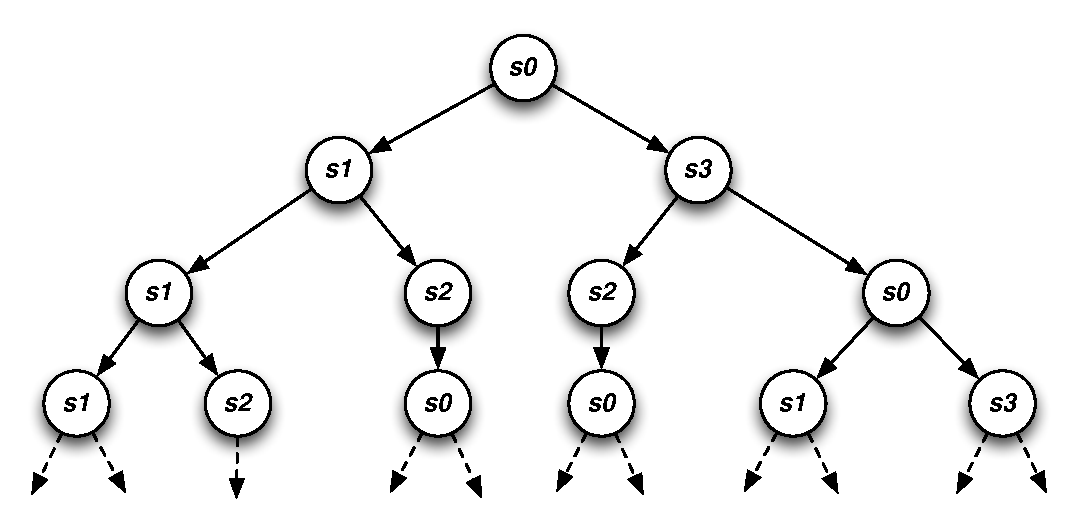
\includegraphics[width=0.8\textwidth]{berechnungsbaum.pdf}
  \end{figure}

  \subsection*{(b) temporale Formeln}
  \begin{enumerate}
    \item Gilt, da $s_0$ direkt $q$ erf�llt.
    \item Gilt nicht, da z.\,B. $s_0 \rightarrow s_1 \rightarrow s_1 \rightarrow \dots$
    \item Gilt nicht, da in $s_1$ weder $p$ noch $q$ gilt.
    \item Gilt, z.\,B. der Pfad $s_0 \rightarrow s_1$. Bis zum ersten Auftreten von $r$ gilt $q$.
    \item Gilt, z.\,B. gilt $r$ in $s_1$.
    \item Gilt, da in $s_0$ schon $q$ gilt und in den Folgezust�nden (egal welcher Pfad gew�hlt wird) jeweils $r$ zum erstem mal Auftritt.
  \end{enumerate}

  \section*{Aufgabe 12.3 - Model Checking CLT}
  \begin{enumerate}[(a)]
    \item $EF(\text{started}\,\, \land \,\,\lnot\text{ready})$
    \item $\text{request} \Rightarrow AF.\text{acknowleged}$
    \item $AF.AG.\text{deadlock}$
  \end{enumerate}
\end{document}
